\section{Progetto di riqualificazione urbana per il Bellinzonese}

\subsection{Introduzione}

\subsection{Ciclopiste}
Durante la pianificazione delle ciclopiste si deve considerare, oltre che della loro funzione di interconnessione, diversi elementi che le rendono a norma, sicure e agibili. Infatti, bisogna tenere conto delle diverse norme che ne regolamentano la creazione. I percorsi ciclabili rappresentano, per i ciclisti, un grosso vantaggio, in quanto separano il traffico lento, da quello a motore, aumentando il confort, la sicurezza e riducendo lo stress. Elementi che si muovono a favore di questo sviluppo sicuro possono essere la segnaletica stradale, pannelli informativi, stampati e internet. Le piste ciclabili possono avere più funzioni, la prima è la mobilità quotidiana (spostamenti funzionali), la seconda è la funzione turistico-ricreativa. Queste due categorie devono essere sviluppate in modo differente, quelle relative allo spostamento quotidiano devono avere un carattere funzionale, efficiente e devono raggiungere i principali centri di lavoro/scolastici; quelli con uno scopo turistico-ricreativo invece non devono rispettare particolari percorsi o destinazioni, in quanto la strada è essa stessa la meta da raggiungere, questi percorsi devono quindi offrire un’esperienza attrattiva con paesaggi e punti di sosta tranquilli. 
La segnaletica, all’interno di un percorso ciclabile, deve permettere di seguire la direzione desiderata senza difficoltà, riducendo al massimo le interruzioni, oltre a ciò ha la funzione di rendere il percorso attrattivo. Grazie ad una buona segnaletica, infatti, le piste diventano più sicure, attrattive e veloci, inoltre diventano più facilmente reperibili, anche da turisti o persone che non sono residenti del posto. 
\\
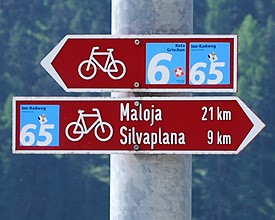
\includegraphics[scale=1]{Capitoli/cartelol.jpg}
\\
Essendo la bici un mezzo di trasporto non dotato di motore, le soste, le deviazioni e in generale gli spostamenti non scorrevoli, implicano una perdita di tempo e soprattutto di energie. Per rendere lo scorrimento di queste piste il più ottimale possibile, l’obiettivo è di minimizzare al massimo il numero di soste durante la percorrenza di una via ciclabile. Problemi che possono influenzare negativamente la qualità del percorso possono essere le geometrie sfavorevoli, topografia sfavorevole, soste di breve/lunga durata (semafori/passaggi a livello). 
Per la creazione della pista ciclabile ottimale, è quindi necessario tenere in considerazione una moltitudine di elementi. 
In Svizzera le piste ciclabili sono rappresentate in colore rosso. Per i percorsi creati nel progetto di riqualifica urbana del territorio bellinzonese, è necessario che la segnaletica sia puntuale e precisa, infatti tutti i nuovi percorsi dovranno essere marcati dettagliatamente e adeguate secondo la regolamentazione consigliata. 
Sempre in più parti del mondo il sistema del traffico viene modificato al fine di permettere l’agevolazione dei mezzi di trasporto lento, un esempio molto prossimo alla nostra realtà, è la nuova struttura della rete stradale di Lugano, che ha permesso ai mezzi di trasporto pubblici e ai ciclisti di coesistere con una maggiore armonia rispetto al precedente modello di rete urbana.  Tuttavia ha scaturito effetti collaterali nei confronti delle abitudini dei conducenti, per questa ragione andrebbero considerate anche queste conseguenze, per prevenire eventuali problemi anche nel territorio in cui si vorrebbe effettuare queste modifiche

\subsection{Traffico bellinzonese, evoluzione dal 1991 al 2017}
Grazie ai dati forniti dall’osservatorio ambientale della Svizzera italiana si può constatare come gli ultimi 20/30 anni abbiamo assistito un importante incremento del traffico. I dati che coprono, generalmente, un periodo che va dal 1991 al 2017, evidenziano la situazione dei nuovi quartieri del comune di Bellinzona. Come si vede dal grafico 1 (la numerazione di grafici e tabelle dovrà essere progressiva e secondo il capitolo, ad esempio 4.1) l’aumento è stato significativo per tutti i punti di rilevamento.  Le cause di questo aumento possono essere varie: aumento della popolazione nelle zone urbane, aumento dei posti di lavori nel quartiere di Bellinzona, incremento del traffico automobilistico e lo sviluppo economico. 
Dare una risposta unica e definitiva è evidentemente difficile ma è chiaro che la pressione del traffico sul centro del nuovo comune è aumentato – oltretutto su una rete stradale che è rimasta praticamente uguale negli ultimi decenni – nonostante le politiche per favorire il trasporto pubblico.
